\chapter{Learner Study}\label{C:lib}

Employing a user study at the early stage of design is an important practice to achieve a better understanding of users and help developers to produce a design that is usable and effective.

In section 2.5, we introduced the concept of persona and presented how it was important in a user centered design. We adopted this technique to represent the target learners in order to provide realistic and help guide the subsequent application design. 

The known information about learners were they were first year engineering and computer science students. Based on this knowledge, we could make some rudimentary assumptions about their ability to use communication technologies offered by smart phones. However, such knowledge did not provide any detailed insights about the learners preferences and abilities in the context of using m-learning application. We therefore began initial investigation to observe our target learners.

We began the observation by launching an online questionnaire to observe learners' attitude towards m-learning and  if the learners had previous experience using text, recorded audio, and video media, communicating through a chat function, performing an electrical assignment, and playing a game-based-learning on smart phones. Next, we performed a statistical analysis on the results and clustered the responses to create personas. Lastly, we evaluated the practicability, and appropriateness of such media and functions. 

Parts of the persona development process have been documented and published within the Proceeding of the \nth{8} International conference on computer Supported Education 
\section{Methodology} 

There were four main stages in this learner study. Firstly, we identified presentation media and learning supported activities grounding on Transactional Distance Theory
\begin{itemize} 
\item Dialogue - smart phones had capability to provide many communication such as message text, e-mail, voice call, and video call. However, with respect to appropriateness of conversation arrangement (i.e., flexible communication schedule for teachers and allow many-to-many communication), we chose text message within a chat application as a communication channel
\item Media presentation - smart phones had capability to deliver learning content to learners using text, recorded audio, and video
\item Learning supported activities - smart phones could provide game-based learning module that allowed the learners to practice what they had learnt and electronic assignments that were used to evaluate their knowledge. 
\end{itemize} 

Secondly, we recruited first year computer engineering, and computer science students from the School of Engineering and Computer Science at the Victoria University of Wellington in New Zealand to participate in our online-based, anonymous questionnaire (see Appendix A). The questionnaire consists of: 
\begin{itemize} 
\item 24 quantitative questions that asked learners to rank their experience and rate their attitude towards the learning supported functions (i.e. chat, game-based learning, and electrical assignment) and presentation media (i.e., text, recorded audio, and video)
\item 4 text box fields that were used to collect free-form, text-based responses on which activities other than calling and texting learners performed on their mobile phones, how they used their mobile phones to support learning, and their m-learning goals. 
\end{itemize}

We conducted the study on October 2015 during the second trimester. From a pool of approximately 150 students, 30 of them completed the survey. Our participants were students who were enrolled in either the Engineering Modelling and Design (ENGR110) or the Introduction to Data Structures and Algorithm (COMP103). They had prior experience in tertiary-level learning because they had passed at least basic computer course either Engineering Technology (ENGR101) which introduced some fundamental technical concepts of engineering electronics, mechatronic, networked, and software systems or Introduction to Computer Program Design (COMP102) which introduced fundamentals of programming in high-level programming language (Java) in the first trimester. Nevertheless, their programming competency had no effect on the observation because the observation variables of experience and attitude towards the learning supported activities and presentation media were not relevant to programming. 

Thirdly, we used five-point Likert scale to rank the experience and measure the attitude. The results were manipulated with two statistical techniques - graphical clustering and k-meaning clustering (Section 3.2). Additionally we listed some interesting findings collected from the free-form text based response (Section 3.3). We used the statistical clustering results and fulfilled it with the qualitative findings to create learner personas. We analyzed reliability of the personas and chose a primary and secondary personas to be used in subsequent stage of m-learning application development. 

Lastly, we concluded the practicability and appropriateness of such learning supported activities and presentation media on smart phones. 

\section{Creating Persona}

We adopted two statistical techniques to create persona: graphical clustering and k-mean clustering  techniques. 

\subsection{Graphical Clustering Technique}
In an attempt to find a behavior pattern from the responses, the responses were plotted on the same graph (Figure 3.1a). The resulting graph was overly distributed and was not effective for determining learners' behavior pattern therefore we performed three rounds of clustering: 

\begin{figure}[!hbt]\centering
    \begin{subfigure}{0.49\textwidth}
 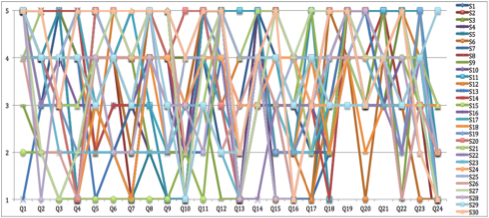
\includegraphics[width=\textwidth]{persona1a}
 \caption{The 30 participants' responses (X-axis represents 24 quantitative questions)}
    \end{subfigure}\hspace{0.01\textwidth}
    \begin{subfigure}{0.49\textwidth}
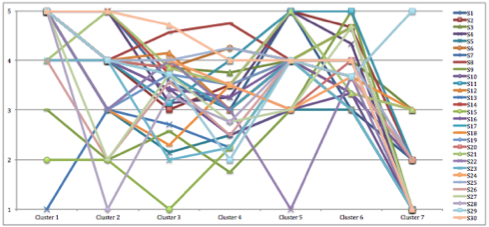
\includegraphics[width=\textwidth]{persona1b}
  \caption{The graph after first round attribute clustering (X axis presents the seven clusters}
    \end{subfigure}
    \begin{subfigure}{0.49\textwidth}
        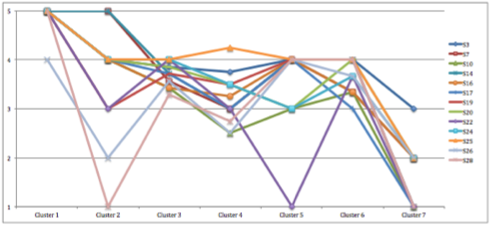
\includegraphics[width=\textwidth]{persona1c}
        \caption{The graph after second round elimination}
    \end{subfigure}\hspace{0.01\textwidth}
\begin{subfigure}{0.49\textwidth}
        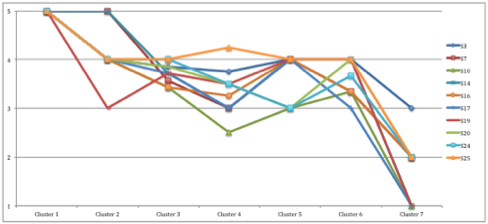
\includegraphics[width=\textwidth]{persona1d}
        \caption{The graph after third round elimination due to extreme values}
    \end{subfigure}
    \caption{Graphical Clustering Process (y-axis presents the responses in the range one to five)}
\end{figure}

\begin{itemize}
\item First Round Attribute Clustering - the questions were divided into seven clusters (i.e., experience in using a mobile phone in daily life, experience in using a mobile phone for educational purpose, experience in using the provided media, experience in using the provided functions, attitude towards m-learning, attitude towards provided functions, and learning preference). For the clusters that consisted of more than one question, the graph was plotted based on their average values (Figure 3.1b).

\item Second Round Elimination - an allowed interval was set based on average value of of each cluster. If a participant provided two or more responses outside the allowed interval, the participant will be removed from the considered group. There were 17 participants excluded as a result (Figure 3.1c). 

\item Third Round Elimination due to Extreme Value - there were three participants who qualified in the second round, but were excluded in this round because their responses to a particular question varied greatly from other participants in the same cluster (Figure 3.1d). 
\end{itemize}

In figure 3.1d, the graph shows a general trend (i.e. these ten participants showed a similar behavior pattern). From the total of 30 participants, only these ten participants were grouped together. The remaining 20 participants were excluded from the final persona creation process. 

Based on the above graphical clustering technique, a persona with a pseudonym "John" was created (Figure 3.4). In order to complete persona John, one of the ten final participants was randomly selected and his/her qualitative responses were fulfilled in persona John's profile.

%%%%%%%%%%%%%%%%%%%%%%%%%%%%%%%%%%%%%%%%%%%%%%%%%

\subsection{K-mean Clustering Technique} 

K-mean clustering is the clustering algorithm partitions all the data (N) into (K) clusters (where K is the number of cluster, chosen before the algorithm starts). The partitioning minimises the sum of squared distances between items and the corresponding centroid (where the centroid is the mean vectors). 


We used Matlab to perform this clustering. 
\begin{enumerate} 
\item Finding appropriate number of cluster (K) using a silhouette plot. The plot illustrated how close each point in one cluster is to the points in the neighbouring clusters. We trialled starting with number of cluster (K) = 2 and increasing the K to 3, 4, 5, 6, and 7 (Figure 3.2). The plots range from +1 to -1. 
\begin{itemize}
\item The closer a cluster is to +1 means it is more distant from its neighbouring clusters. That is to say, the cluster is appropriated partitioned)
\item The closer a cluster is to -1 means the data is probably partitioned into the wrong cluster 
\end{itemize}

In figure 3.2, only two plots show non-negative value where k = 3 and 4 (Figure 3.2b and 3.2c). Therefore, at this point, 3 and 4 clusters were the appropriate number of clusters. However, when the number of cluster k=3, most of its points had larger silhouette value comparing to cluster k=4. Ultimately, we chose to dived the data into 3 clusters. 

\item Arranging the participants (N=30)  into 3 clusters (K=3) using mean clustering function in Matlab. The results were: 
\begin{itemize}
\item Cluster 1 consisted of seven participants: P4, P5, P13, P15, P18, P23 and P28
\item Cluster 2 consisted of six participants: P9, P19, P20, P22, P26 and P27
\item Cluster 3 consisted of 17 participants: P1, P2, P3, P6, P7, P8, P10, P11, P12, P14, P16, P17, P21, P24, P25, P29 and P30 
\end{itemize}

\item Seeking for the most appropriate participant from each cluster to represent the rest of the participant in the same cluster by calculating Euclidean Distance between each participant and the average value using Matlab. The participant who has the lowest Euclidean will be chosen as the representative (Figure 3.3). 
\item Fulfilling the qualitative responses of the selected participant in the persona

\end{enumerate}
We used pseudonym "Annie", "Stephen", and "Clara" to represent cluster 1, 2, and 3 persona respectively. Based on the clustering, cluster 3 had the highest number of participants, therefore Clara was chosen as a primary persona. Meanwhile cluster 1 and 2 had less number of participants, therefore Annie and Stephen were secondary personas. 

\newpage 
\begin{figure}[!hbt]\centering
    \begin{subfigure}{0.45\textwidth}
 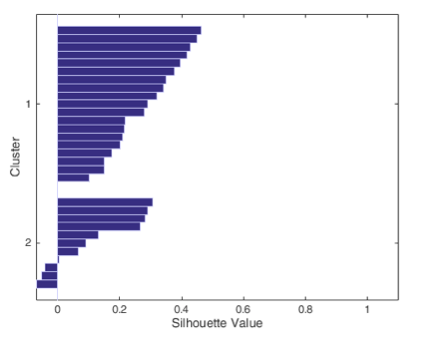
\includegraphics[width=\textwidth]{persona3a}
 \caption{Silhouette Value when K=2}
    \end{subfigure}\hspace{0.01\textwidth}
    \begin{subfigure}{0.45\textwidth}
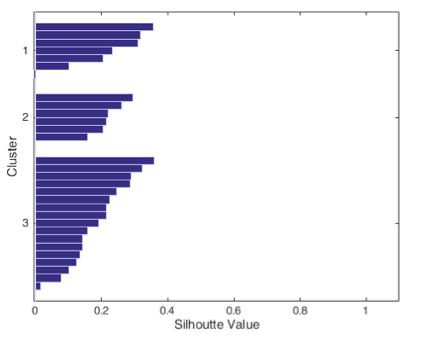
\includegraphics[width=\textwidth]{persona3b}
  \caption{Silhouette Value when K=3}
    \end{subfigure}
    \begin{subfigure}{0.45\textwidth}
        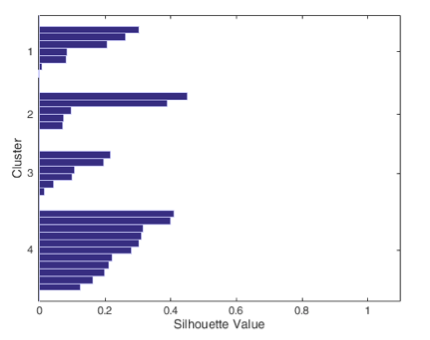
\includegraphics[width=\textwidth]{persona3c}
        \caption{Silhouette Value when K=4}
    \end{subfigure}\hspace{0.01\textwidth}
\begin{subfigure}{0.45\textwidth}
        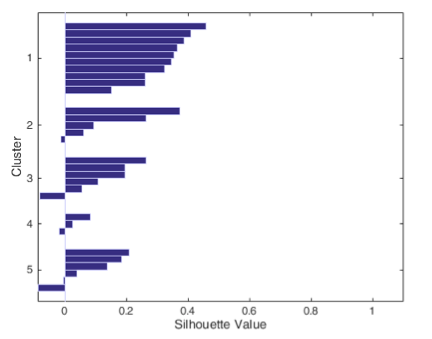
\includegraphics[width=\textwidth]{persona3d}
        \caption{Silhouette Value when K=5}
    \end{subfigure}
 \begin{subfigure}{0.45\textwidth}
 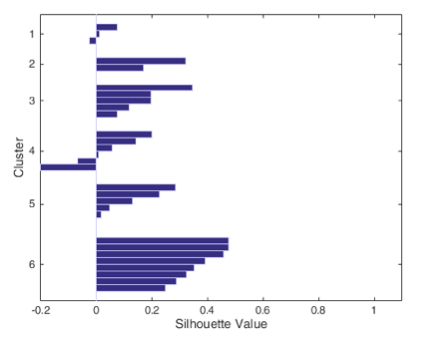
\includegraphics[width=\textwidth]{persona3e}
 \caption{Silhouette Value when K=6}
    \end{subfigure}\hspace{0.01\textwidth}
    \begin{subfigure}{0.45\textwidth}
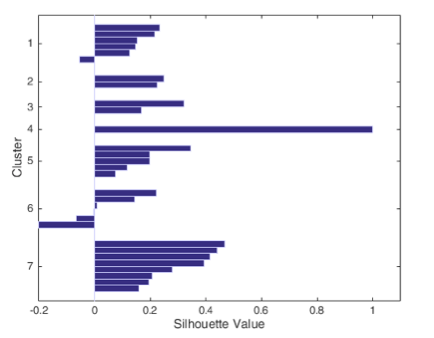
\includegraphics[width=\textwidth]{persona3f}
  \caption{Silhouette Value when K=7}
    \end{subfigure}
    \caption{Silhouette plots to find the appropriate number for cluster (K)}
\end{figure}

\newpage
\begin{figure}[!hbt]\centering
    \begin{subfigure}{1\textwidth}
 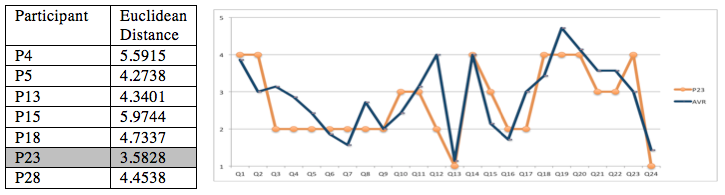
\includegraphics[width=\textwidth]{persona4a}
 \caption{P23 was chosen as the representative for cluster 1}
    \end{subfigure}
    \begin{subfigure}{1\textwidth}
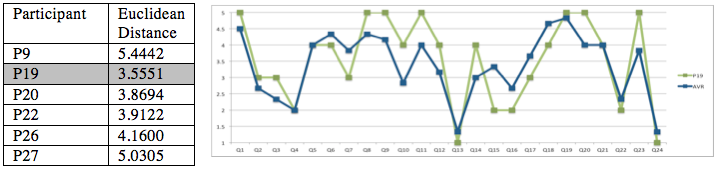
\includegraphics[width=\textwidth]{persona4b}
  \caption{P19 was chosen as the representative for cluster 2}
    \end{subfigure}
    \begin{subfigure}{1\textwidth}
        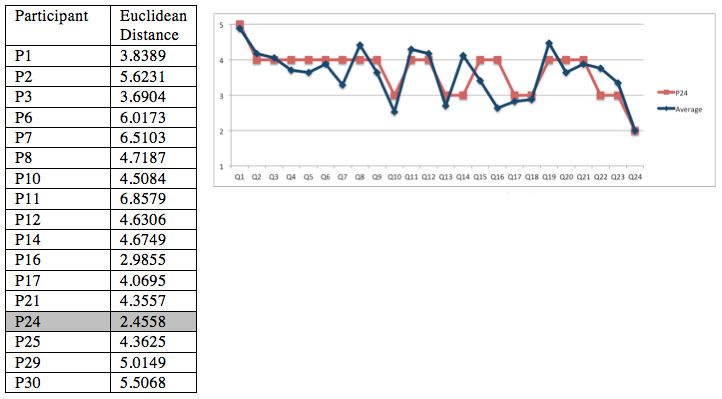
\includegraphics[width=\textwidth]{persona4c}
        \caption{P24 was chosen as the representative for cluster 3}
    \end{subfigure}
    \caption{The most appropriated participant to represent the rest of the participants in its cluster}
\end{figure}

%%%%%%%%%%%%%%%%%%%%%%%%%%%%%%%%%%%%%%%%%%%%%%
\newpage 
\section {Persona Results}

This section presents four persona: one persona (John) was created from graphical clustering technique and three persona (Annie, Stephen, and Clara) were created from K-meaning clustering technique. We had permission to use all the people images presented in the personas' profile. Figure 3.4 presents persona John which was created from graphical presentation technique and Figure 3.5, 3.6, and 3.7 present Annie, Stephen and Clara personas which were created from K-mean clustering technique. 

There was a concern towards the graphical clustering technique as it eliminated and neglected more than half of the participants in its result. The persona John was created based on eight participants out of a pool of 30 participants. The remaining twenty-two participants were excluded. On the other hand, comparing to the graphical clustering, the K-mean clustering technique was able to better arrange all the participants into its appropriated clusters and none of the participants were excluded in its clustering process. Hence, we only took three personas (Annie, Stephen, and Clara) into account and highlighted Clara as the primary persona. 


\newpage 
\begin{figure}[!hbt]
\centering
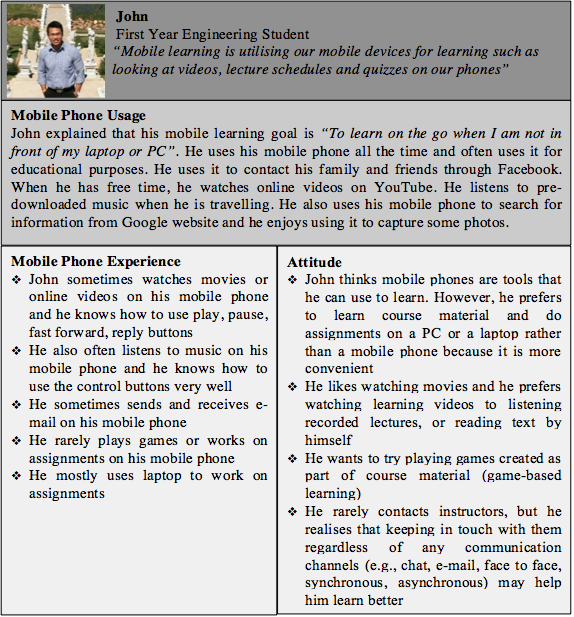
\includegraphics[width=1 \textwidth]{persona2}
\caption{John persona created with graphical clustering technique}
\end{figure}


\newpage 
\begin{figure}[!hbt]
\centering
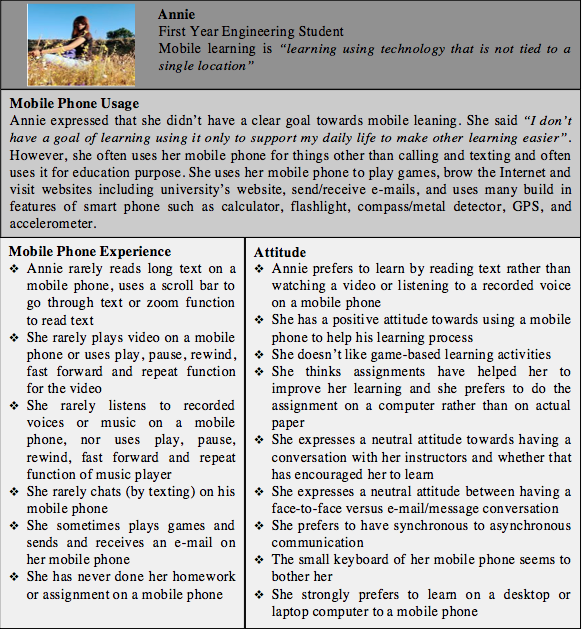
\includegraphics[width=1.0 \textwidth]{annie}
\caption{Annie persona (secondary) created with K-mean clustering technique}
\end{figure}
\newpage 
\begin{figure}[!hbt]
\centering
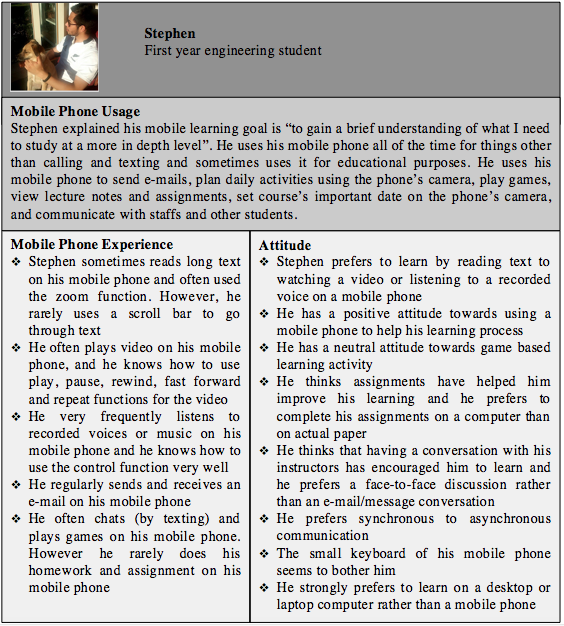
\includegraphics[width=1.0 \textwidth]{stephen}
\caption{Stephen persona (secondary) created with K-mean clustering technique}
\end{figure}
\newpage
\begin{figure}[!hbt]
\centering
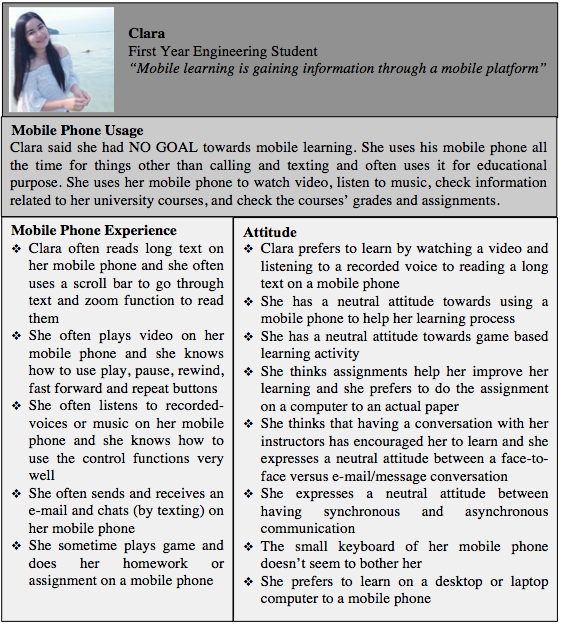
\includegraphics[width=1.0 \textwidth]{clara}
\caption{Clara persona (primary) created with K-mean clustering technique}
\end{figure}


\newpage 
\section{Qualitative Findings}

This section summarized some interesting qualitative findings. 

\subsection{Mobile Phones Usages} 
Participants were also asked to list the activities that they performed on their mobile phones other than calling and texting. The following list shows the usage categories:

\begin{enumerate}
\item Communication - they used their mobile phones to access social media websites (e.g., Facebook\footnote{https://www.facebook.com}, Reddit\footnote{https://www.reddit.com}, and sending and receiving e-mails

\item Entertainment - they used their mobile phones to watch video online from video-sharing websites (e.g., YouTube), listen to music, and play games

\item Research - participants mentioned that they accessed Google whenever they wanted to find any information. They also read news, and participated in online-forums on their mobile phones

\item Personal Management - they used many basic functions available on their mobile phones to manage their daily life. For example, they used note function to list activities to be completed, calendar to receive notifications for when these tasks should be completed, alarm clock to wake them up in the morning, and they managed their bank account online

\item Other - they mentioned many others basic functions of mobile phones (e.g., flash light, map, camera) which they used regularly
\end{enumerate}

When the usage of mobile phones was specified to "educational purposes'', the interesting findings were:

\begin{enumerate}
\item They used their mobile phones to access social media websites, then contact their classmates to discuss their lessons and assignments
\item They also downloaded lecture notes, slides, and videos and used these downloaded materials from their mobile phones when they were away from university
\item For research purposes, they read articles on their mobile phones and used online search engines (i.e., Google) when they had questions and wanted to find more information
\item They visited the school's website to keep themselves updated, and accessed learning resources via University's Blackboard system
\item They used mobile phones' basic functions such as clock, calendar, and note to help them to manage their learning schedule, and they also used their camera to capture their lecture notes
\end{enumerate}

\subsection{Mobile Learning Goals} 
Learning goal was another interesting focus area, as it could inspire and motivate learners to learn. Firstly, we asked the participants to explain the term ``mobile learning'' in order to observe their initial understanding towards the term which inferred if they could set their m-learning goal. Most of them showed that they understood the term and could differentiate m-learning from other types of learning. For example a student answered that 
\newline 
\begin{addmargin}[1.5em]{1.5em}
\textit{``Mobile learning to me is being able to gain and apply knowledge anywhere at anytime including when an internet connection is unavailable''}
\end{addmargin}\hfill

Other learners also mentioned learning on the go, learning anywhere, and convenient when they were not stationary. 

When the participants were asked to identify their goals of learning on mobile phone. Most of them considered mobile phones as tools to help them to learn outside of their classrooms when they were not in front of their laptop or computer. Examples of the answers were: 
\newline 
\begin{addmargin}[1.5em]{1.5em}
\textit{``I do not consider myself a person who learns from a mobile phone, only one who uses it for time management and organising my learning, which comes from other sources unless it is an extreme scenario (i.e. there are absolutely no computers available to me)''}
\end{addmargin}

\hfill
\begin{addmargin}[1.5em]{1.5em}
\textit{``I just want to be able to find out what I need to know very quickly. ...''}
\end{addmargin}\hfill 



\section{Analysis}

Based on the primary persona (Clara) profile, the target learners had previous experiences using the text, recorded audio, and video as well as knew how to, for example play, pause, and fast forward, use the control functions. These presentation media seemed to be practically feasible for them. Among the observed learning support activities, chat function seemed to have the highest feasibility because they appreciated that communication with their teachers would help improve their learning and they had already familiar with texting and emailing on the mobile devices. On the other hand, despite being appreciated that assignment had helped improve their learning, they preferred to do it on a desktop computer or laptop rather than a mobile phone. These results supported the idea that the learners did not take m-learning as a primary source of learning. In addition, they had neutral attitude towards the game-based learning. Therefore, some strategies may be needed in order to encourage them to complete the electrical assignment and participate in the game-based learning. Rewarding techniques and sending notifications to them can be used in this matter.


The qualitative findings supported the idea that mobile phone was a powerful tool for supporting ubiquitous learning. Its use as an educational tool was now very much an established part of our target learners' daily learning environment. However, they did not set up a learning goal even though they adopted the phones for many learning activities. It raised awareness about learners' m-learning acceptance and that encouragements and promotions may be required. 

\section{Summary}

In order to ensure that text, recorded audio, and video presentation media and chat, gram-based learning, and electrical assignment learning-supported activities could contribute an effective m-learning application for our target learners, a learners study was carried out. A total of 30 participants, 26 male and four female, who were first year computer engineering and computer science students at the Victoria University of Wellington in New Zealand answered an online-based questionnaire. 

Based on the statistical manipulation and qualitative findings, we created a primary persona Clara which represented majority of the target learners. Clara had prior experience towards the presentation media therefore the media seemed to be practically feasible for m-learning design. Similarly, she was familiar with the chat function and had positive attitude towards this communication activity. On the other hand, the game-based learning and electrical assignment seemed to require some encouragements and promotions. Besides, the primary persona, in order to ensure that our design catered all target learners, we created another two secondary personas: Annie and Stephen. These personas would be used to inform user-centered design in the next m-learning development process. 

Based on the qualitative findings, the participants have been using their mobile phone in their daily lives. The main mobile phone usage categories comprised of communication, entertainment, research, and personal management. These usage had also been applied within educational context. However, they did not have a cleared goal towards m-learning, hence encouragement and promotion may be required to promote m-learning. 









